\chapter[Minería de Datos]{Minería de Datos}
\label{ch:dm}

\section{Minería de Datos}

El proceso de minería de datos o exploración de datos es un proceso, considerado una etapa de un proceso mayor llamado ``Descubrimiento de Conocimiento en Base de Datos'' (KDD, del inglés, Knowledge Discovery in Databases), ``proceso no trivial de identificar patrones válidos, novedosos, potencialmente útiles y comprensible a partir de los datos''. \footnote{Fayyad et al. 1996}\\

Usualmente ambos conceptos son intercambiables, pero se entiende por KDD al proceso de encontrar información y/o patrones útiles en los datos. En cambio minería de datos, es el uso de algoritmos para extraer información y/o patrones derivados dentro del proceso KDD.\\


Dentro de la definición del proceso KDD se pueden desprender los siguientes conceptos:

\begin{itemize}
    \item Patrones válidos:
     Los patrones deben ser precisos y verdaderos para nuevos datos, similar al principio de inducción matemática.
    \item Novedosos:
    Los datos deben aportar algo nuevo al usuario, un conocimiento. Esto es la esencia de la minería de datos.
    \item Útil:
    Los datos deben conducir a acciones por parte de los usuarios receptores.
    \item Comprensible:
    Los datos deben ser posible de interpretar y por ende comunicar.
\end{itemize}

En la Figura \ref{fig:kdd}, se puede apreciar el proceso de KDD.\\

\begin{figure}[H]
\begin{minipage}{\textwidth} 
\centering 
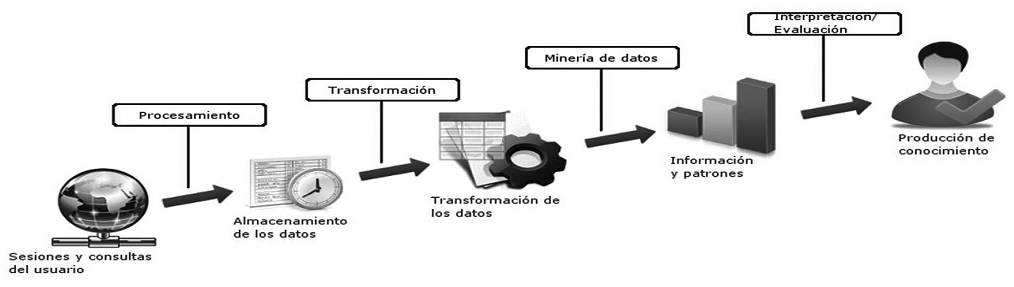
\includegraphics[width=10cm,height=5cm] {kdd.png} 
\caption[Proceso KDD]{Proceso KDD~\footnote{Imagen extraída de http://www.scielo.org.co articulo ``Aplicación del proceso de KDD en el contexto de bibliomining: El caso Elogim''}}
\label{fig:kdd}
\end{minipage}
\end{figure}

\subsection{Fases del Descubrimiento del Conocimiento}

El proceso KDD puede ser representado en 7 objetivos, los cuales se logran en diferentes fases, estos objetivos son:

\begin{enumerate}
    \item Determinar las fuentes de información que pueden ser útiles y dónde conseguirlas.
    \item Diseñar un esquema de almacenamiento de datos, un Data Warehouse.
    \item Implementación del almacén de datos que permita la navegación y visualización previa de los datos para el análisis.
    \item Selección, limpieza y transformación de los datos a analizar.
    \item Seleccionar y aplicar el método de minería de datos apropiado.
    \item Evaluación, interpretación, transformación y representación de los patrones extraídos.
    \item Difusión y uso del nuevo conocimiento.
    
\end{enumerate}

\subsubsection{Recogida de Datos}

La primeras fases del KDD determinan que las fases sucesivas sean capaces de extraer conocimiento válido y útil a partir de la información original.\\

En la fase de recogida de datos se sigue los siguientes pasos:

\begin{itemize}
    \item Selección de datos: 
    Por lo general la información que se quiere investigar sobre un cierto dominio de la organización se encuentra en bases de datos y fuentes internas como externas.
    \item Pre-proceso o limpieza de datos:
    En este paso se debe eliminar el mayor número de datos erróneos o inconsistentes e irrelevantes, esto también se conoce como limpieza y selección.
    \item Transformación de datos:
    Una vez limpiados y seleccionados los datos, se realiza un proceso de transformación que permite homologar la información, dando como resultado un conjunto de filas y columnas denominado ``Vista Minable'', con el fin de dejar los datos preparados para la modelización.
\end{itemize}

\subsubsection{Modelamiento}

El modelamiento o minería de datos es la etapa principal del KDD, aquí se determinan patrones y modelos para descubrir el conocimiento. Existen dos tipos de modelos y diferentes tareas para cada modelo.

\begin{enumerate}
    \item Tareas del Modelo Predictivo\\
    Son aquellas que buscan patrones que ayuden a predecir el comportamiento o tendencia de uno o varios valores.\\
    
    \begin{itemize}
        \item Clasificación:
        Los datos o registros son agrupados en clases, los cuales pueden tomar valores discretos. Su objetivo es determinar patrones en los registros, para identificar o predecir a que clase pertenecen los registros nuevos.
        
        \item Regresión:
        Se usa una regresión para predecir los valores ausentes de una variable basándose en su relación con otras variables del conjunto de datos.
    \end{itemize}
    
    \item Tareas del Modelo Descriptivo\\
    Son aquellas que exploran las propiedades de los datos analizados para encontrar patrones entre ellos.\\
    
    \begin{itemize}
        \item Agrupamiento (Clasificación no supervisada):
        Es similar a la clasificación, excepto que los grupos no son predefinidos. El objetivo es segmentar un conjunto de datos en grupos que pueden ser disjuntos o no. Los grupos se forman basados en la similaridad de los datos en ciertas variables. Como los grupos no son dados a priori se debe dar una interpretación de los grupos que se forman.
        
        \item Correlaciones:
        Identifica el grado de similitud de dos variables numéricas.
        \item Asociación:
        Las asociaciones entre dos atributos ocurre cuando la frecuencia de que se den dos valores determinados de cada uno conjuntamente es relativamente alta.
        \item Reglas de asociación secuenciales:
        Es una variante de asociación que utiliza la variable tiempo para identificar correlación.

        
    \end{itemize}
    
\end{enumerate}


Para estos modelos y tareas existen diferentes técnicas de minería de datos las cuales se pueden aplicar, a continuación se muestra un cuadro de las técnicas y tareas que utilizan, Figura \ref{fig:tecnicas}


\begin{figure}[H]
\begin{minipage}{\textwidth} 
\centering 
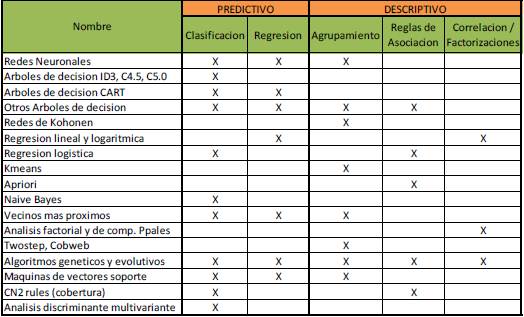
\includegraphics[width=12cm,height=7cm] {tecnicas.png}
\caption[Técnicas de minería de datos]{Técnicas de minería de datos~\footnote{Imagen extraída del libro ``Introducción a la Minería de Datos'', pag. 148, cap. 6}}
\label{fig:tecnicas}
\end{minipage}
\end{figure}

\subsubsection{Evaluación}

La fase de evaluación tiene como objetivo probar y validar el modelo creado en las fases anteriores. Para realizar las pruebas del modelo, se divide el set de datos en dos grupos, un grupo de entrenamiento de los datos, que ayuda a identificar la predicción que se espera, y el otro grupo es de prueba se valida la predicción y se analiza el porcentaje de acierto de dicha predicción. Por lo general se obtienen varios modelos aplicando las diferentes técnicas de minería de datos, los cuales son comparados buscando aquel que se ajuste mejor al problema. Si ninguno de los modelos alcanza los resultados esperados, debe
alterarse alguno de los pasos anteriores para generar nuevos modelos.

\section{Técnicas de Minería de Datos}

En el capitulo anterior se explico que existen diferentes técnicas y tareas en minería de datos para los distintos tipos de modelamiento.\\

El modelamiento acorde a este trabajo, corresponde a un modelo predictivo, en el cual se utilizarán cuatro técnicas en \textit{RapidMiner}, para generar cuatro modelos, estas técnicas son:\\

\begin{itemize}
	\item Regresión Lineal:\\
Es una técnica utilizada para la predicción numérica. Es una medida estadística que determina la relación ente una variable dependiente y una serie de variables independientes.\\
La regresión lineal intenta modelar la relación entre una variable escalar y una o más variables explicativas ajustando una ecuación lineal a los datos observados. Por ejemplo, uno podría querer relacionar los pesos de los individuos con sus alturas usando un modelo de regresión lineal \cite{rl}.

	\item Árboles de decisión:\\

Es una representación de datos que tiene forma de árbol invertido, donde sus nodos raíces están en la parte superior, creciendo hacia abajo.\\
Su objetivo es predecir el valor de un atributo destino (generalmente llamado clase o etiqueta) basándose en varios atributos de entrada, cada nodo interior del árbol corresponde a uno de los atributos de entrada. El número de aristas de un nodo interior nominal es igual al número de valores posibles del atributo de entrada correspondiente. Los bordes salientes de los atributos numéricos están etiquetados con rangos disjuntos. Cada nodo de hoja representa un valor del atributo de etiqueta dado los valores de los atributos de entrada representados por el camino de la raíz a la hoja \cite{ad}.
	\item Redes Neuronales:\\

Una red neuronal, es un modelo matemático o modelo computacional que se inspira en la estructura y aspectos funcionales de las redes neuronales biológicas. Una red neuronal consiste en un grupo interconectado de neuronas artificiales, y procesa la información utilizando un enfoque conexionista a la computación (el principio conexionista central es que los fenómenos mentales pueden ser descritos por redes interconectadas de unidades simples ya menudo uniformes). En la mayoría de los casos, una red neuronal es un sistema adaptativo que cambia su estructura basada en información externa o interna que fluye a través de la red durante la fase de aprendizaje. Las redes neuronales modernas suelen usarse para modelar relaciones complejas entre entradas y salidas o para encontrar patrones en los datos \cite{redn}.

	\item Máquinas de Vectores de Soporte (SVN):\\

Las máquinas de vectores de soporte estándar toman un conjunto de datos de entrada y predice, para cada entrada dada, cuál de las dos clases posibles comprende la entrada, haciendo del SVM un clasificador binario no probabilístico lineal. Dado un conjunto de ejemplos de entrenamiento, cada uno marcado como pertenecientes a una de dos categorías, un algoritmo de entrenamiento de SVM construye un modelo que asigna nuevos ejemplos en una categoría u otra. Un modelo SVM es una representación de los ejemplos como puntos en el espacio, mapeados de modo que los ejemplos de las categorías separadas se dividan por una brecha clara que es lo más amplia posible. Nuevos ejemplos se asignan a ese mismo espacio y se predice que pertenecen a una categoría basada en qué lado de la brecha en la que caen \cite{svn}.

\end{itemize}  
















